%%%%%%%%%%%%%%%%%% NON LINEAR PLATE VIBRATION (PULSE) %%%%%%%%%%%%%%%%%%

\newcommand{\NLPlateVibrationzero}[1]
{   
	\onecontour{ xlabel = $x$, ylabel = $y$, colormap/bluered, point meta max=0.01, point meta min=-0.007}{21}
	%
	{./doc/chapters/IBVPP_BVP/figures/Non_Linear_Cartesian_Plates_Pulse/U0.dat}{}{ #1 }
}

\newcommand{\NLPlateVibrationOne}[1]
{   
	\onecontour{ xlabel = $x$, ylabel = $y$, colormap/bluered,  point meta max=0.01, point meta min=-0.007}{21}
	%
	{./doc/chapters/IBVPP_BVP/figures/Non_Linear_Cartesian_Plates_Pulse/U1.dat}{}{ #1 }
}

\newcommand{\NLPlateVibrationTwo}[1]
{   
	\onecontour{ xlabel = $x$, ylabel = $y$, colormap/bluered,  point meta max=0.01, point meta min=-0.007}{21}
	%
	{./doc/chapters/IBVPP_BVP/figures/Non_Linear_Cartesian_Plates_Pulse/U2.dat}{}{ #1 }
}

\newcommand{\NLPlateVibrationThree}[1]
{   
	\onecontour{ xlabel = $x$, ylabel = $y$, colormap/bluered, point meta max=0.01, point meta min=-0.007}{21}
	%
	{./doc/chapters/IBVPP_BVP/figures/Non_Linear_Cartesian_Plates_Pulse/U3.dat}{}{ #1 }
}

\newcommand{\NLPlateVibrationFour}[1]
{   
	\onecontour{ xlabel = $x$, ylabel = $y$, colormap/bluered, point meta max=0.01, point meta min=-0.007}{21}
	%
	{./doc/chapters/IBVPP_BVP/figures/Non_Linear_Cartesian_Plates_Pulse/U4.dat}{}{ #1 }
}




\newcommand{\NLPlateStresszero}[1]
{   
	\onecontour{ xlabel = $x$, ylabel = $y$, colormap/bluered, point meta max=5.8e-6, point meta min=-7.5e-7}{21}
	%
	{./doc/chapters/IBVPP_BVP/figures/Non_Linear_Cartesian_Plates_Pulse/F0.dat}{}{ #1 }
}

\newcommand{\NLPlateStressOne}[1]
{   
	\onecontour{ xlabel = $x$, ylabel = $y$, colormap/bluered, point meta max=5.8e-6, point meta min=-7.5e-7}{21}
	%
	{./doc/chapters/IBVPP_BVP/figures/Non_Linear_Cartesian_Plates_Pulse/F1.dat}{}{ #1 }
}

\newcommand{\NLPlateStressTwo}[1]
{   
	\onecontour{ xlabel = $x$, ylabel = $y$, colormap/bluered, point meta max=5.8e-6, point meta min=-7.5e-7}{21}
	%
	{./doc/chapters/IBVPP_BVP/figures/Non_Linear_Cartesian_Plates_Pulse/F2.dat}{}{ #1 }
}

\newcommand{\NLPlateStressThree}[1]
{   
	\onecontour{ xlabel = $x$, ylabel = $y$, colormap/bluered, point meta max=5.8e-6, point meta min=-7.5e-7}{21}
	%
	{./doc/chapters/IBVPP_BVP/figures/Non_Linear_Cartesian_Plates_Pulse/F3.dat}{}{ #1 }
}

\newcommand{\NLPlateStressFour}[1]
{   
	\onecontour{ xlabel = $x$, ylabel = $y$, colormap/bluered, point meta max=5.8e-6, point meta min=-7.5e-7}{21}
	%
	{./doc/chapters/IBVPP_BVP/figures/Non_Linear_Cartesian_Plates_Pulse/F4.dat}{}{ #1 }
}


%%%%%%%%%%%%%%%%%% DEVELOPER FIGURES %%%%%%%%%%%%%%%%%%%%%%
\newcommand{\IBVPandBVPmethodlines}
{
\begin{figure}[H]
	\centering
	\begin{tikzpicture}
	\tikzstyle{every node}=[align=center]
	\node(d) at ( 1.5,-10.5 ) {Temporal \\ discretization};
	\node(e) at ( 1.5, -3.5 ) {Spatial \\ discretization};
	
	\tikzstyle{every node}=[draw, align=center, rectangle ]
	
	\node(a) at (0,0) {\textbf{IBVP} + \textbf{BVP} \\ \\
		$ \dfrac{\partial u}{\partial t} = \mathcal{L}_u(\vect{x},t,u,v),$\\ \\ $u(x,0)=u_0(x), $ \\ \\
		$ \mathcal{L}_v(\vect{x},t,v,u)= 0,$   \\ 
		+ \\ 
		$\eval{h_u(\vect{x},t,u)}_{\partial \Omega} = 0. $ \\ $\eval{h_v(\vect{x},t,v)}_{\partial \Omega} = 0.$};
	
	\node(b) at (0,-7) {
        \hspace{-1.5cm} \textbf{ Step 1. Boundary points} $ U_{\partial \Omega}$  \\ \\
         $ \eval{H_U(U;t)}_{\partial \Omega} = 0, $ \\  \\
        \hspace{-3.2cm} \textbf{Step 2. BVP } for $ V$ \\ \\
        $ F_V(V,U;t)= 0, $ \\ \\
       	$ \eval{H_V(V;t)}_{\partial \Omega} = 0. $ \\ \\
        \textbf{Step 3. IBVP: Spatial discretization}\\ \\
		$ \dfrac{\dd U_{\Omega}}{\dd t} = F_{U}(U,V;t), $ \quad  
		$ U(0)=U^0, $ \\  
		  };
	
	
	\node(c) at (0,-14) {\textbf{Step4. Temporal scheme} \\ \\
		$ G({U}_{\Omega}^{n+1}, {U}^{n}, \ldots {U}^{n+1-s};t_n, \Delta t)= F_U(U^n, V^n; t_n), $ \\ \\
		$ F_V(V^n,U^n;t_n)= 0, $ \\ 
		+ \\ 
		$ \eval{H_U(U^n;t_n)}_{\partial \Omega} = 0, $ \\ 
		$ \eval{H_V(V^n;t_n)}_{\partial \Omega} = 0. $ 
		\\ \\ where $U^0$ is known.};
	\foreach \from/\to in {a/b,b/c}
	\draw [->, thick = 1 pt] (\from) -- (\to) ;
	
	\end{tikzpicture}
	\caption{Method of lines for mixed initial and boundary value problems.}
	\label{fig:IBVPPandBVPmethodlines}
\end{figure}
}
\newcommand{\IBVPandBVPalgorithm}
{
\begin{figure}[H]
	\hspace{-0.5cm}
	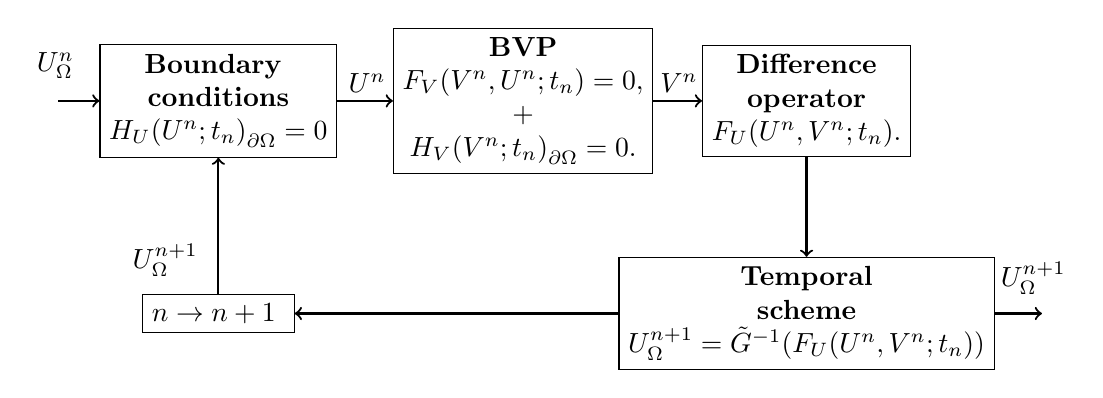
\begin{tikzpicture}[scale=0.9]
	\node[rectangle](0) at (-2.4,0) {};
	\node[rectangle](0un) at (-2.3,0.5) {$U_{\Omega}^{n}$};
	\node[rectangle](f) at (11.76,-3) {};
	\node[rectangle](un1) at (11.5,-2.5) {$U_{\Omega}^{n+1}$};
	\node[rectangle](e) at (-0.75,-2.25) {$U_{\Omega}^{n+1}$};
	\node(ab) at (2.1,0.25) {${U^n}$};
	\node(bc) at (6.5,0.25) {${V^n}$};
	
	\tikzstyle{every node}=[draw, align=center, rectangle ]
	\node(a) at (0,0) {\textbf{Boundary } \\ \textbf{conditions} \\ 
		$\eval{H_U(U^n;t_n)}_{\partial \Omega} = 0 $};
	
	\node(b) at (4.3,0) {\textbf{BVP} \\ $ F_V(V^n,U^n;t_n)= 0, $ \\ 
		+ \\ 
		$ \eval{H_V(V^n;t_n)}_{\partial \Omega} = 0 $.};
	
	\node(c) at (8.3,0) {\textbf{Difference} \\ \textbf{operator} \\ $ F_U(U^n,V^n; t_n)$.};
	
	\node(d) at (8.3,-3) {\textbf{Temporal} \\ \textbf{scheme} \\ $U_{\Omega}^{n+1} = \tilde{G}^{-1}(F_U(U^n,V^n; t_n))$ };
	
	\node(e) at (0,-3) {$n \rightarrow n +1 $ };
	
	
	\foreach \from/\to in {0/a,a/b,b/c,c/d,d/e,e/a,d/f}
	\draw [->, thick = 1 pt] (\from) -- (\to) ;
	\end{tikzpicture}
	\caption{Algorithm for mixed initial and boundary value problems.}
	\label{fig:IBVPandBVPalgorithm}
\end{figure}
}